\chapter{KiCAD}

\noindent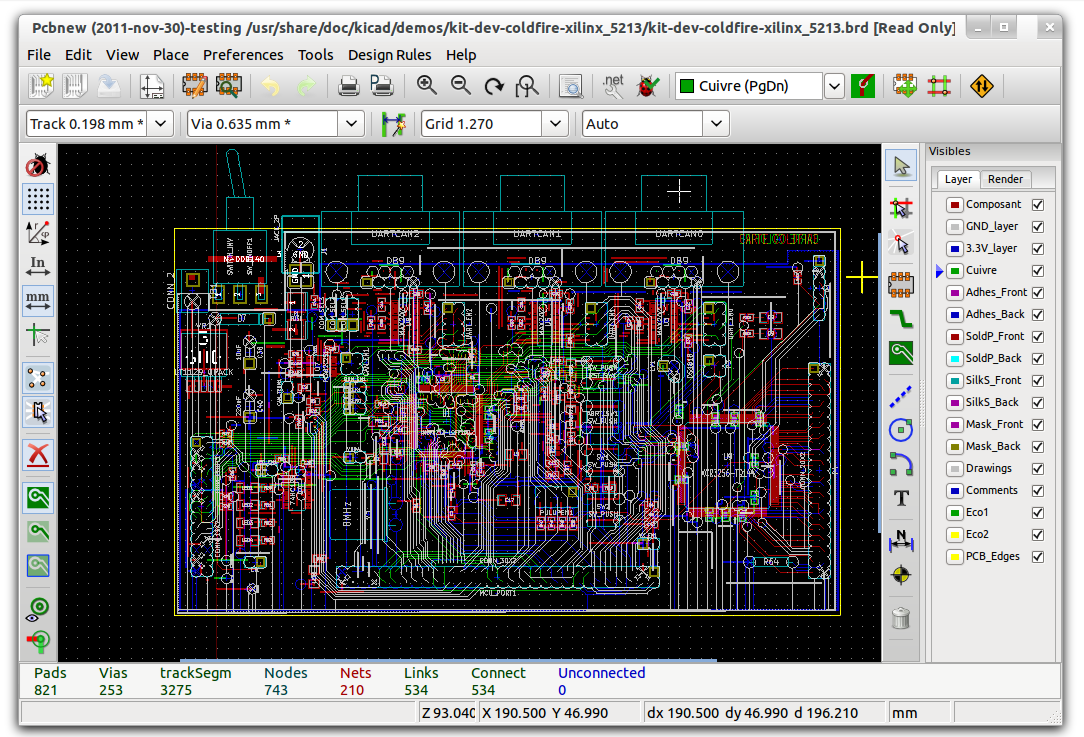
\includegraphics[height=0.5\textheight]{kicad/kicad_pcbnew.png}


\cp{http://ru.wikibooks.org/wiki/KiCad}

KiCad\ --- распространяемый по лицензии GNU GPL программный комплекс САПР EDA с
открытыми исходными текстами, предназначенный для разработки электрических схем
и печатных плат.

Кроссплатформенность компонентов KiCad обеспечивается использованием 
библиотеки wxWidgets. Поддерживаются операционные системы Linux, 
Windows NT 5.x, Free\-BSD и Solaris.

Разработчик\ --- Жан-Пьер Шарра (фр. Jean-Pierre Charras), исследователь 
в LIS (фр. Laboratoire des Images et des Signaux\ --- Лаборатория Изображений 
и Сигналов) и преподаватель электроники и обработки изображений в фр. 
IUT de Saint Martin d’Hères (Франция).

\cp{http://ru.wikibooks.org/wiki/KiCad/Miniurok}

Этот раздел познакомит Вас с основами использования системы KiCad. Он содержит
информацию о всех шагах создания простой печатной платы: от рисования
электрической схемы до печати готового рисунка платы. Вам будут представлены
различные возможности KiCad и предложены эффективные пути решения различных
задач.

Руководство пользователя, поставляемое вместе с KiCad, содержит значительно
больше информации, чем этот урок. Ознакомтесь с ним, чтобы узнать больше об
использовании программы.



\secrel{Установка}\secdown

\secrel{\win}\label{kicadinstwin}

\menu{\winr{\url{http://www.kicad-pcb.org/}}>Download>\winstart}

\menu{\winr{\url{http://kicad.nosoftware.cz/}}>
\file{KiCad\_testing\-201x.xx.xx-BZRxxxx\_Win\_full\_version.exe}}

\bigskip

\menu{Installer Language>\emph{English}>Ok} 
в русифицированном инсталляторе кривые шрифты

\menu{KiCAD 20xx.xx.xx Setup>Next}

\menu{Лицензия>Agree}

\menu{Components>\checkbox\ все>Next}

\menu{Location>\file{C:/KiCad}>Install}

\menu{Completing Setup>\uncheckbox Wings3D>Finish}

\secrel{\linux}\label{kicadinstlin}

\begin{verbatim}
root# aptitude install kicad-doc-ru kicad
\end{verbatim}

\lst{+++\ $\sim$/.blackbox/menu}{}{/tmp/kicad.bbmenu}

\secrel{Настройка библиотек}

Для добавления библиотек, поставляемых с этой книгой, сделайте \emph{git
clone} или \emph{git pull}:

\begin{verbatim}
user:~$ git clone --depth=1 -o gh https://github.com/ponyatov/odurino.git odurino
user:~$ cd odurino
user:~/odurino$ git pull
\end{verbatim}

\menu{\prog{kicad}>\prog{eeschema}>Настройки>Библиотека}

\menu{Пользовательские пути поиска>Добавить>\file{/home/user/odurino/lib}}

\menu{Файлы библиотек>все стандартные>Удалить>OK}

\menu{Файлы библиотек>Добавить>R,L,C,SPICE,DA\_POWER,..>Открыть>OK}

\bigskip
Для проверки работы библиотек можете открыть проект

\menu{\prog{kicad}>Файл>Открыть>\file{~/Azbuka/bcollis/led1/led1.pro}}

или сразу схему

\menu{\prog{eeschema}>Файл>Открыть>\file{~/Azbuka/bcollis/led1/led1.sch}}

\secrel{Дотфайлы}

Посколько программа изначально писалась как юниксовая, пользовательские
настройки хранятся в dot-файлах:

\lst{~/.kicad}{}{kicad/kicad.dotfile}

\begin{description}
\item[KicadFrame*] размеры и положение окна менеджера проектов
\item[WorkingDir] каталог с текущим рабочим проектом
\item[fileN] список последних проектов (\ \menu{Файл>Последние файлы}\ )
\end{description}

\lst{~/.eeschema}{}{kicad/eeschema.dotfile}

\begin{description}
\item[SchematicFrame*] размеры и положение окна \prog{eeschema}
\item[fileN] список последних схем (\ \menu{Файл>Последние файлы}\ )
\end{description}

\secrel{Глобальные шаблоны}\label{kicadtemplates}

После установки \kicad\ можно скорректировать файлы глобальных шаблонов, чтобы
новые проекты создавались сразу с нужными настройками, прежде всего с нужным
нам набором библиотек:

\begin{verbatim}
sudo vim /usr/share/kicad/template/kicad.pro
\end{verbatim}

\lst{/usr/share/kicad/template/kicad.pro}{}{kicad/kicad.template}

\begin{description}
\item[LibDir] каталог библиотек, установите на свой или корпоративный/групповой
\item[LibNameN] задается список библиотек по умолчанию, приопишите ваш типовой
набор
\item[eeschema/libraries] схемные библиотеки \eeschema
\item[pcbnew/libraries] библиотеки надстеков для печатных плат \pcbnew
\end{description}

\secup



\secrel{\prog{eeschema}: редактор электрических схем}

обеспечивает:

\begin{itemize}
\item создание однолистовых и иерархических схем,
\item проверку их корректности ERC (контроль электрических правил),
\item создание списка электрических цепей netlist для редактора топологии платы
pcbnew или для spice-моделирования схемы, 
\item доступ к документации на используемые в схеме электронные компоненты
(datasheet).
\end{itemize}


\secrel{Библиотеки компонентов}\secdown

\cp{http://habrahabr.ru/post/197582/}\bigskip

Модель компонента в САПР EDA состоит из следующих частей:

\begin{itemize}
  \item условное графическое обозначение (УГО) для схемного редактора
  \item модель компонента для редактора печатных плат (ПП)
  \item модель для симулятора (SPICE)
  \item 3D модель для передачи в универсальный САПР для работы с конструкцией
  \item дополнительные пользовательские данные: индексы компонента для
  заказа у разных поставщиков, ссылки на документацию, и т.п.
\end{itemize}

Части могут иметь несколько вариантов, например два варианта УГО (ГОСТ и ISO),
три корпуса (DIP, PLCC и LQFP), две модели для симулятора (идеальная и с
учетом паразитных эффектов), и 2 механических модели (габаритный кубик, и
подробная).

Кроме того, часто в один корпус упаковывается несколько одинаковых или разных
элементов. Одинаковые\ --- 2--4 операционных усилителя (ОУ), или вентили
логики. Разные\ --- части вакуумной лампы, разнесенные на схеме по разным
каскадам.

\bigskip

В составе KiCad поставляются библиотеки электронных компонентов (обычных и
поверхностно монтируемых SMD). Для многих библиотечных компонентов есть
3D-модели, созданные в \prog{Wings3D}.

Но как только вы начинаете работать со свежеустановленным KiCADом, тут же
обнаруживается, что библиотечные компоненты или не подходят\note{например не
соответствуют ГОСТ или стандартам предприятия}, или нужных компонентов попросту
нет в библиотеках.

Рассмотрим последовательное создание совершенно нового элемента на примере
модуля USB интерфейса HEX\_FT2232RL \ref{HEXFT2232RL}

\secrel{Создание УГО для схем}

Нам необходим встроенный редактор символов схем (библиотечных компонентов),
запускаем его следующим образом:

\begin{enumerate}
  \item Вначале запускаем \file{eeschema}
  \begin{itemize}
    \item[вверху] меню и панель инструментов
    \item[слева] область размерности и шага сетки редактора (настройка рабочей
    области)
    \item[справа] область элементов схем и перемещения по иерархии схемы
  \end{itemize}
  \item Далее запускаем встроенный
  \menu{Редактор библиотек}\ 
\includegraphics[height=2em]{kicad/ee22.png}

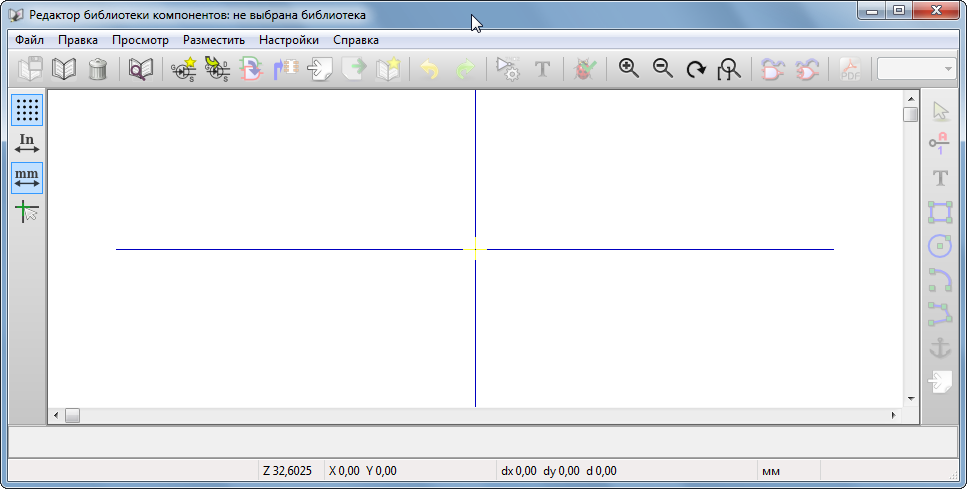
\includegraphics[height=0.5\textheight]{kicad/lib23.png}
\end{enumerate}

Необходимо создать новую библиотеку и первый собственный компонент:

\menu{Создать новый компонент}
\includegraphics[height=2em]{kicad/newel.png},

\menu{Свойства компонента>Общие Настройки},

\menu{Имя компонента>HEX\_FT232RL}

\menu{Обозначение по умолчанию>U}

\menu{Количество элементов в корпусе>1}

\menu{OK}
\bigskip

В верхней панели инструментов активировались несколько кнопок, выбираем

\menu{Сохранить текущий компонент в новой библиотеке}

\includegraphics[height=2em]{kicad/lib26.png}

В открывшемся диалоге выберите каталог для библиотеки
\file{/home/user/kicad/}, и укажите имя файла (новой) библиотеки
\menu{\file{MyModules}>Сохранить}.

\bigskip
Теперь нужно добавить созданную библиотеку в рабочий список.
\bigskip

Настроим дополнительный путь, где лежат файлы библиотек. Это могут быть ваши
личные библиотеки, специальная библиотека для конкретного проекта, или комплект
библиотек поставляемых вместе с этой книгой: выберите в меню
\menu{Настройки>Библиотека}, \menu{Пользовательские пути
поиска>добавить>\file{/home/user/kicad/}}, \menu{Ok}.

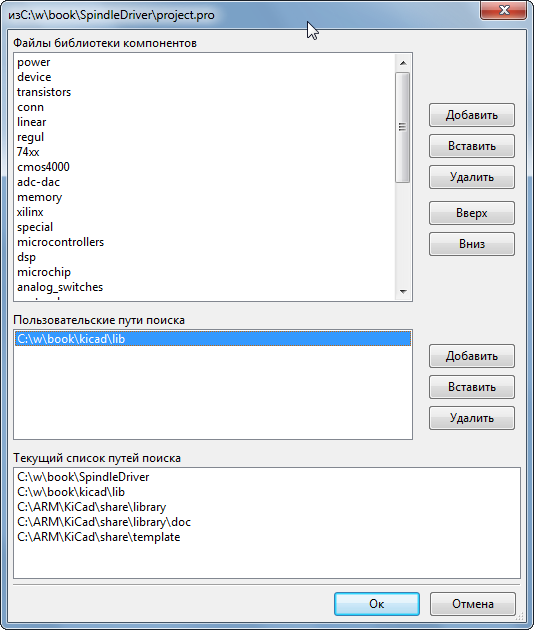
\includegraphics[height=0.5\textheight]{kicad/lib25.png}

\menu{Настройки>Библиотека},
\menu{Файлы библиотеки компонентов>power>\lms>Вставить}.
Выбираем только что созданную библиотеку \file{MyModules}.
Она будет вставлена в список до выбранной \file{power}.

\bigskip
Проделанные настройки применятся только к текущему проекту. Если Вы хотите 
чтобы новая библиотека всегда добавлялась к новым проектам, вам нужно добавить
новый путь поиска библиотек и ее название в файл шаблона, как это описано в
\ref{kicadtemplates}.

\bigskip
Если вы хотите изменить только что созданное или уже сущесствующее УГО, нужно
выбрать рабочую библиотеку, ту библиотеку в которой мы хотим работать (создавать
или редактировать компоненты). На панели инструментов нажимается кнопка

\menu{Выбор рабочей библиотеки}
\includegraphics[height=2em]{kicad/lib24.png},

\menu{Выбрать библиотеку>MyModules>Ok}.

Загружаем созданный ранее (пустой) компонент \file{HEX\_FT232RL} (или любой
другой)

\menu{Загрузить компонент для редактирования}
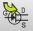
\includegraphics[height=2em]{kicad/editel.png}

\menu{Выбор компонента>Список всех>Элементы>\file{HEX\_FT232RL}>Ok}

\bigskip
\includegraphics[height=0.45\textheight]{odurino/usb/HEXFT232RL.png}

Сейчас у нас элемент не имеет графических элементов, и состоит только из
нескольких текстовых полей с обозначениями, слепленных в одной точке. Нужно их
растащить: \rms, САПР не может различить близкие элементы и уточняет для
какого поля мы хотим контекстное меню. Выбираем любое, \menu{Переместить поле}\
или кнопка \keys{M}. Перетаскиваем элемент, и \lms\ на свободном месте.

Пользуясь \ref{eskd}, отрисовываем на освободившемся месте УГО элемента,
пользуясь кнопками на панели справа. Рисование выполняется по сетке, шаг
выбирается \menu{\rms>Выбор сетки}, набор сеток фиксированный (?). При рисовании
ГОСТовских УГО округляем до ближайших дюймовых размеров\footnote{\ 1mil=1/1000
дюйма, 100mil=2.54mm=типовой шаг DIP микросхем}, или в меньшей сетке если нужно
точно гостовские размеры.

УГО имеет \term{точку привязки}, относительно которой отрисовываются элементы.
На практике важно то, что вокруг этой точки элемент вращается. Для перемещения
этой точки можно использовать кнопку

\menu{Переместить точку привязки}
\includegraphics[height=2em]{kicad/lib27.png}.

Добавляем выводы компонента: \menu{Добавить вывод
компонента}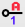
\includegraphics[height=2em]{kicad/lib28.png}.

\bigskip
Например для резистора создание выводов будет выглядеть вот так:

\bigskip
\menu{Свойства вывода}

\menu{Имя>A}

\menu{Номер>1}

\menu{Ориентация>Вправо}

\menu{Электр.тип>Пассивный}

\menu{Размер шрифта>1.27мм}

\menu{Длина>2.54мм}

\menu{Ok}

\bigskip

\menu{Имя>B}

\menu{Номер>2}

\menu{Ориентация>Влево}

\menu{Ok}

\bigskip
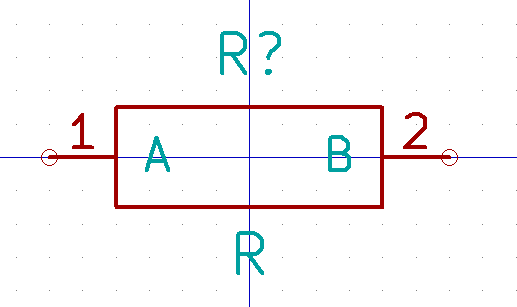
\includegraphics[height=0.5\textheight]{kicad/lib29.png}
\bigskip

Сохраняем библиотеку: \menu{Сохранить текущую
библиотеку}
\includegraphics[height=2em]{kicad/lib30.png}

\menu{Подтверждение>Включая последние изменения компонента?>Да}

\menu{Подтверждение>Компонент существует. Изменить его?>Да}

\menu{Подтверждение>Изменить файл библиотеки ?>Да}

\secrel{Модель печатной платы}

Модель печатной платы в программе \pcbnew\ состоит из нескольких
\termdef{слоев}{слой печатной платы} с разными функциями, для типичной
двухслойной ПП:

\begin{itemize}
  \item верх
  \begin{description}
  \item[Front] медь верхнего слоя
  \item[Adhes\_Front] карта нанесения клея для компонентов
  \item[SoldP\_] карта нанесения паяльной пасты
  \item[SilkS\_] шелкография: маркировка элементов, надписи, и т.п.
  \item[Mask\_] паяльная маска 
  \end{description}
  \item низ
  \begin{description}
  \item[Back] медь нижнего слоя
  \item[Adhes\_Back] карта нанесения клея для компонентов 
  \end{description}
  \item контуры
  \begin{description}
  \item[Контур ПП] слой определяющий физ.геометрию платы, используется при
  фрезеровке контуров, сверлении монтажных отверстий, разделке сверловкой и т.п.
  \item[Пояснения] вспомогательная текстовая информация
  \item[Чертеж] вспомогательная графическая информация: габаритные размеры, зоны
  монтажа,..
  \end{description}

\item В зависимости от технологии производства и пожеланий разработчика могут
добавляться любые дополнительные слои.
\end{itemize}

\secrel{Создание падстека}

\termdef{Падстек}{падстек}\ --- модель контактной площадки компонента, в виде
набора геометрий отдельно для каждого \term{слоя} печатной платы. Также включает
информацию о диаметре сверления.

% \secrel{PS:}
% 
% Компоненты и посадочные места корпусов можно ассоциировать с документацией,
% ключевыми словами и осуществлять быстрый поиск компонента по функциональному
% назначению.
% 
% \secup
% 
% \secru{Отрисовка схемы (часть 2)}
% 
% \secdown
% 
% \secru{Автоматическое обозначение элементов}
% 
% Автоматическое обозначение элементов и перенумерация выполняется кнопкой\\
% \menu{Обозначить компоненты на
% схеме}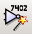
\includegraphics[height=2em]{kicad/ee000004.png}
% 
% \secru{Генерация списка цепей}
% 
% Список цепей (нетлист) используется для передачи информации о соединении
% компонентов между программами. Чаще всего СЦ создается после отрисовки схемы для
% передачи данных в программу трассировки печатной платы (ПП).

\secup


\secrel{\prog{gerbview}: просмотр фотошаблонов}

позволяет просматривать Gerber-файлы перед передачей печатных плат в
производство.



\chapter{Использование SPICE}
\cp{http://www.mithatkonar.com/wiki/doku.php/kicad/kicad\_spice\_quick\_guide}

\section{Доступные SPICE-пакеты}

\begin{itemize}
\item \href{http://ngspice.sourceforge.net/}{ngspice}: Arguably the most FOSSy
commonly available SPICE engine.
\item
\href{https://www.gnu.org/software/gnucap/}{gnucap}\note{уже включен в
виндозную сборку KiCAD}:
Not actually SPICE but tries to be syntax-compatible.
\item \href{http://www.spiceopus.si/}{SpiceOpus}: Proprietary but nice,
especially the output plotting.
\item \href{http://www.linear.com/designtools/software/}{LTSpice}: Linear
Technology's popular, proprietary Windows solution.
Works in \href{http://www.winehq.org/}{Wine}. Has a GUI anyway, so … ? Whether
it's scritable needs to be verified.
\item
\href{http://www.cadence.com/products/orcad/pspice_simulation/Pages/default.aspx}{PSpice}:
Windows-only, expensive, defacto standard professional solution in the USA. They
also have a tradition of making available a \emph{gratis} crippleware student
version.
Also has a \underline{GUI}, so … ?
\item \url{http://www.ngspice.com/}\ --- on-line вариант \prog{ngspice}, удобен
для начального обучения
\item Какие-то еще?
\end{itemize}

\section{Установка \prog{ngspice} под \win}

\menu{\winr\url{http://ngspice.sourceforge.net/download.html}>\prog{ng-spice-rework}>\file{ngspice-xx\_xxxxxx.zip}}

\section{Установка \prog{ngspice} под \linux}

\begin{verbatim}
root# aptitude install ngspice
\end{verbatim}

\section{Библиотеки компонентов со SPICE-элементами}

\begin{itemize}

\item There is a library of basic SPICE components that ships with KiCad. It's
good enough for initial experimentation.

\begin{itemize}
\item The library isn't included in Eeschema projects by default. You'll have to
add it manually if you want to use it.
In Debian-based Linux, it's at \\/usr/share/kicad/library/pspice.lib. (PSpice is
a popular proprietary version of SPICE.)
\end{itemize}

\item I am developing (very slowly)
\href{https://bitbucket.org/mithat/kicad-spice-library}{my own
library}\note{Mithat Konar \email{webs@mithatkonar.com}}
of components based on the above with some changes and additions.

\end{itemize}

\subsection{Настройка проекта}

\begin{enumerate}
\item Create a new project in the conventional way.
\item Open Eeschema and remove all the library references included by default.
\item Manually add one or more libraries with SPICE components to the project.
\begin{itemize}
  \item Note that the SPICE library that comes packaged with KiCad is not
  included by default in new KiCad projects.
\end{itemize}
\item Specify the SPICE engine you want to use:
\begin{itemize}
  \item Click the “Generate netlist” button (or the equivalent menu item).
  \item Select the “Spice” tab
  \item Enter the name of the command to invoke the simulator (with or without
path) in the “Simulator command:” textbox.
\end{itemize}
\end{enumerate}

\subsection{Making it happen}

\begin{enumerate}
  \item
Do your schematic capture, subject to a couple best practices:
\begin{itemize}
  \item
For named nets, use global labels instead of local labels.
\begin{itemize}
  \item
The reason for this is that in the netlists, global identifiers will be used
as-is but local labels get text prepended to the name—which makes it hard for
you to remember/guess what the full identifier is.
\end{itemize}
Use the ”0” component from a SPICE component library rather than the GND symbol.
\begin{itemize}
  \item
”0” is the official name of ground node in SPICE. Some engines may translate GND
into 0, some may not.
\end{itemize}
\end{itemize}
  \item
Specify the simulations you want to run and the output you want to display by
adding a text block (i.e., “comment”) with the needed SPICE and Nutmeg syntax
plus a little added mojo. To do an AC analysis and plot the response at node
\verb|vout|, you would add the following block:
\begin{lstlisting}
+PSPICE
.control
ac dec 66 1kHz 120kHz
plot vdb(vout)
set units = degrees
plot vp(vout)
.endc
\end{lstlisting}
\begin{itemize}
  \item
The line +PSPICE is KiCad-speak for, “Stick the following text at the end of a
SPICE netlist.”
\begin{itemize}
  \item
\textcircled{!} There appears to be a bug in the parser that requires you to add
a space after +PSPICE and before the line break.
\end{itemize}
  \item
There is a corresponding -PSPICE that is KiCad-speak for, “Stick the following
text at the start of a SPICE netlist.”
  \item
If you don't like seeing references to PSpice in your designs, you can use
+GNUCAP and -GNUCAP instead. I believe they are exact synonyms in this context,
but I am not certain.
  \item
Yes, this means you need to learn some
\href{http://newton.ex.ac.uk/teaching/cdhw/Electronics2/userguide/sec5.html}{SPICE
and Nutmeg} syntax. It's not hard.
\end{itemize}
  \item
Run the simulation:
\begin{itemize}
  \item
Click the “Generate netlist” button (or the equivalent menu item).
  \item
Select the “Spice” tab, and make sure “Default format” is checked. (You should
only have to do this once; it will just save you time in subsequent invocations
of the dialog.)
  \item
Click the “Run simulator” button.
\end{itemize}
\end{enumerate}


\section{Программа \prog{Wings3D} для создания 3D моделей}

Эта программа может вам пригодиться если вы планируете создавать 3D модели для PCB элементов.

Архив и файлы документации (Linux и Windows) в папке kicad/wings3d.

Взгляните на домашнюю страницу Wings3D чтобы узнать подробнее о программе.

pcbnew использует файлы в формате wrml (.wrl) экспортируемые из Wings3D (родной формат Wings3D - это .wings).

\subsection{Установка \prog{Wings3D} под \win}

\menu{\winr{\url{http://www.wings3d.com/}}>Downloads>Stable Release>\win
(32/64b)}

\menu{file{wings-n.n.n.exe}}

\menu{Compononets>\checkbox QuickLaunch>Next}

\menu{Location>\file{C:/Program Files/wings3d\_n.n.n}>Next>Install>Close}% 


% \secrel{KiCAD}

% \cp{http://ru.wikibooks.org/wiki/KiCad/Miniurok}
% 
% Этот раздел познакомит Вас с основами использования системы KiCad. Он содержит
% информацию о всех шагах создания простой печатной платы: от рисования
% электрической схемы до печати готового рисунка платы. Вам будут представлены
% различные возможности KiCad и предложены эффективные пути решения различных
% задач.
% 
% Руководство пользователя, поставляемое вместе с KiCad, содержит значительно
% больше информации, чем этот урок. Ознакомтесь с ним, чтобы узнать больше об
% использовании программы.
% 
% 
\cp{http://ru.wikibooks.org/wiki/KiCad}

KiCad\ --- распространяемый по лицензии GNU GPL программный комплекс САПР EDA с
открытыми исходными текстами, предназначенный для разработки электрических схем
и печатных плат.

Кроссплатформенность компонентов KiCad обеспечивается использованием 
библиотеки wxWidgets. Поддерживаются операционные системы Linux, 
Windows NT 5.x, Free\-BSD и Solaris.

Разработчик\ --- Жан-Пьер Шарра (фр. Jean-Pierre Charras), исследователь 
в LIS (фр. Laboratoire des Images et des Signaux\ --- Лаборатория Изображений 
и Сигналов) и преподаватель электроники и обработки изображений в фр. 
IUT de Saint Martin d’Hères (Франция).

\cp{http://ru.wikibooks.org/wiki/KiCad/Miniurok}

Этот раздел познакомит Вас с основами использования системы KiCad. Он содержит
информацию о всех шагах создания простой печатной платы: от рисования
электрической схемы до печати готового рисунка платы. Вам будут представлены
различные возможности KiCad и предложены эффективные пути решения различных
задач.

Руководство пользователя, поставляемое вместе с KiCad, содержит значительно
больше информации, чем этот урок. Ознакомтесь с ним, чтобы узнать больше об
использовании программы.


% 
% \secdown
% 
% \secen{Installing KiCAD}
\secru{Установка KiCAD}
\label{kicadinstall}

\bigskip
\menu{
\wcmd{
\url{http://www.kicad-pcb.org/}
}>Download>KiCAD for OS }

\bigskip\menu{\file{KiCad\_stable-2013.07.07-BZR4022\_Win\_full\_version.exe}}

\bigskip

\menu{Installer Language>Russian>Ok}

\menu{Установка KiCAD 2013.07.07>Далее}

\menu{Лицензия>Принимаю}

\menu{Компоненты>\checkbox\ все>Далее}

\menu{Папка установки>\file{D:/ARM/KiCad}>Установить}

\menu{Копирование файлов}

\menu{Завершение установки>\checkbox\ Wings3D>Готово}

\bigskip

\wcmd{\url{http://www.wings3d.com/}>Downloads>Stable>Windows (32b)}

\bigskip\menu{\file{wings-1.5.3.exe}}

\bigskip

\menu{Wings 3D 1.5.3 Setup>Next}

\menu{Install Location>\file{D:/ARM/Wings3D}>Next}

\menu{Start Menu Folder>Install}

\menu{Completed>Close}




% 
% \section{Создание проекта в менеджере проектов \prog{kicad}}

В верхней части панели \term{менеджера проектов} \prog{kicad}
имеются большие кнопки запуска компонентов KiCad:

\begin{itemize}
\item \icoesch\ \prog{EeSchema}\ --- Редактор принципиальных схем
\item
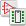
\includegraphics[height=0.1\textheight]{tmp/icon_cvpcb.png}\
\prog{CvPcb}\
--- Программа редактирования падстеков (отверстий и площадок)
\item 

\includegraphics[height=0.1\textheight]{tmp/icon_pcbnew.png}
\prog{Pcbnew}\ ---
Редактор печатных плат
\item

\includegraphics[height=0.1\textheight]{tmp/icon_gerbview.png}
\prog{GerbView}\ --- Программа просмотра фотошаблонов в формате Gerber
\item \prog{Bitmap2Component}\ --- Создание компонента из черно-белого
изображения (например логотипа)
\item 
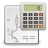
\includegraphics[height=0.1\textheight]{tmp/icon_pcbcalculator.png}
\prog{PcbCalculator}\ --- Калькулятор для печатных плат
\item 
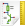
\includegraphics[height=0.1\textheight]{tmp/icon_pagelayout.png}
\prog{PageLayout}\ --- редактор формата листа схемы
\end{itemize}

Каждая кнопка запускает соответствующую программу. Мы будем использовать эти
программы по мере изучения.

\bigskip
Лучше всего для каждого проекта использовать раздельные папки; в противном
случае система может сбиться с толку, если файлы из разных проектов будут лежать
в одной папке. Проделайте следующие шаги:

\begin{enumerate}
  \item Создайте папку проекта \file{D:/ARM/SpindleDriver}
  \item Запустите программу KiCad
  \item Создайте проект (project)
  \begin{itemize}
    \item 
На панели инструментов KiCad выберите левую иконку с подсказкой\\
\menu{Начать новый проект}, используйте команду меню
\menu{Файл>Новый>Пустой} или сочетание клавиш \keys{Ctrl+N}.
    \item 
В диалоге \menu{Создать новый проект} выберите созданную папку
выберите только что созданную папку \file{D:/ARM/SpindleDriver} и
введите имя проекта \menu{\file{SpindleDriver}} и нажмите \menu{Сохранить}.
	\item
Если папка проекта содержит какие-то файлы, будет выведено окно выбора:
создать подпапку с именем проекта \menu{Yes}, или записать файл проекта
в указанную папку как есть \menu{No}. Нажмите No.
    \item 
Сохраните проект кнопкой \menu{Сохранить текущий проект}, \menu{Файл>Сохранить}
или \keys{Ctrl+S}.
	\item
В папке появится файл \file{SpindleDriver.pro}, содержащий установки вашего 
проекта. Файл имеет тектовый формат, поэтому при необходимости его можно открыть
в любом редакторе и вручную аккуратно подправить, например скорректировать
настройки зазоров печатной платы.
  \end{itemize}
\end{enumerate}

\section{Создание принципиальной схемы в \prog{eeschema}\ (часть 1)}

Запустите редактор принципиальных схем, нажав на панели KiCad большую кнопку
\icoesch.

При первом запуске \prog{eeschema}\ стартует с новым проектом и
показывает предупреждение, что файла схемы еще нет. Просто нажмите \menu{ОК}.

Если вас не устраивает черный фон рабочец области или цвета элементов схемы,
поменяйте настроки цветов \menu{Настройки>Цвета}. 

На правом краю окна редактора схем есть вертикальная панель инструментов,
которые мы и будем использовать для рисования схемы. Этими инструментами можно
выбирать объекты, размещать компоненты, вводить связи и т.д.

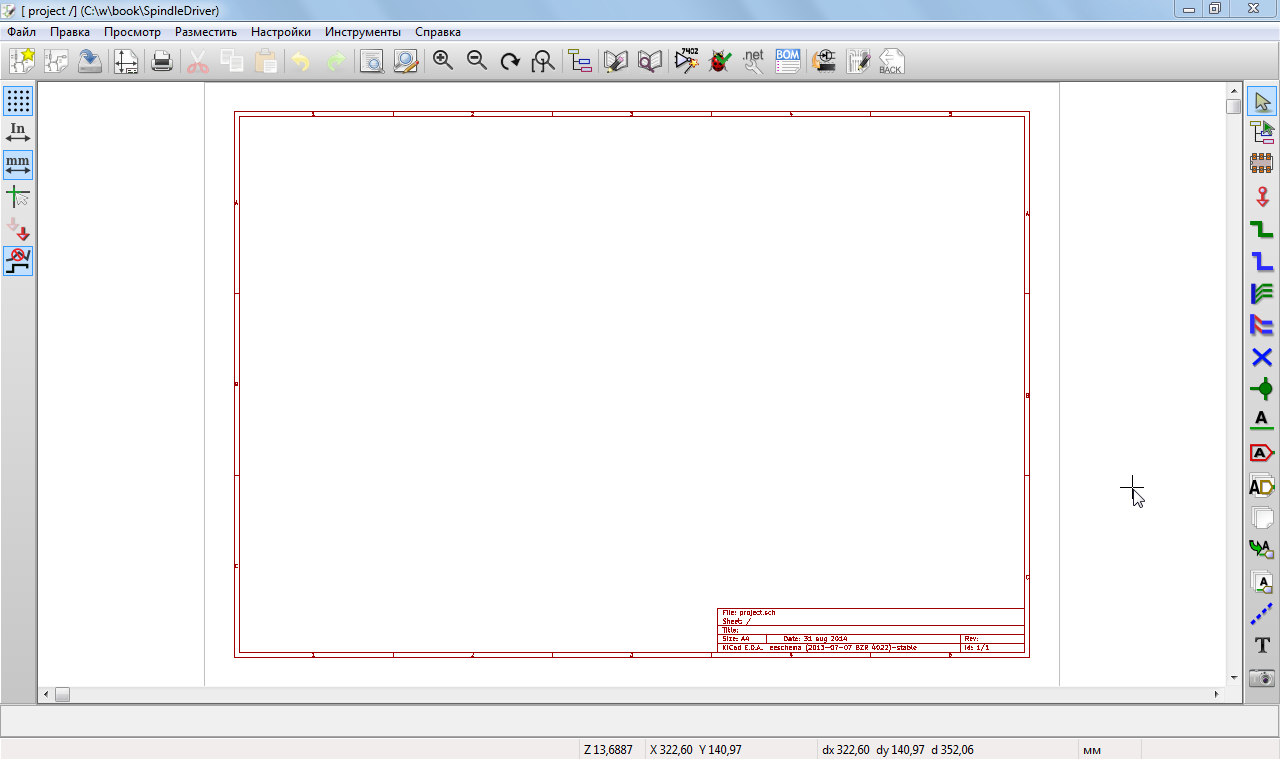
\includegraphics[width=0.9\textwidth]{kicad/ee15.png}

Завершение работы инструмента: вы можете выбрать другой инструмент из правой
инструментальной панели или же указать \menu{Отложить инструмент} по правому
клику мышки \keys{\rms}.

\section{Инструмент \emph{Добавить компоненты}}

\begin{itemize}
  \item 
На правой панели нажмите кнопку \menu{Разместить компонент}\
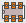
\includegraphics[height=2em]{kicad/ee21.png}. Курсор изменится со стрелки на
карандаш. Удобнее использовать сочетание клавиш \keys{Shift+A}.
Кликните в поле схемы чтобы начать размещение компонента. Появится диалог
\menu{Выбор компонента}. Вы можете выбрать компонент несколькими путями:
  \item
  \begin{enumerate}
    \item 
Если вы знаете точное имя копонента, введите его в поле \menu{Имя}, а
затем нажмите \keys{Enter} или \keys{OK}.
    \item 
Если вы знаете имя только приблизительно, в поле \menu{Имя} введите шаблон для
поиска, например, \menu{*BD*}, затем нажмите \keys{Enter} или \keys{OK}. Вы
увидите окно \\\menu{Выбрать компонент} со списком найденных компонентов.

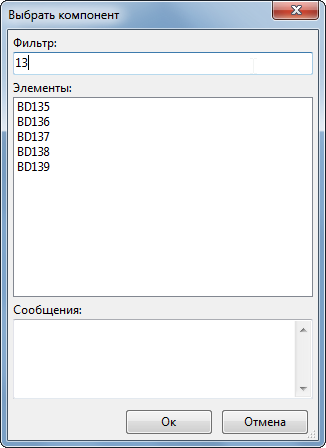
\includegraphics[height=0.5\textheight]{kicad/ee16.png}
    \item 
Вы можете искать компонент по ключевому слову, введя его в поле \menu{Имя},
затем кликнув \menu{Поиск по ключевому слову}. Однако на данный момент качество
библиотек все еще низкое, и немногие компоненты имеют ключевые слова, поэтому
эта возможность полезна косвенно.
    \item 
Можно выбрать недавно использованные компоненты из \menu{Списка истории}.
    \item 
Кнопка \menu{Список всех} вызывает диалог, в котором можно выбрать сначала
библиотеку \menu{74xx}, а затем ее компонент \menu{74HCT04}.
    \item 
Кнопка \menu{Выбор просмотром} вызывает \menu{Обзор библиотек}, позволяя
просмотреть библиотеки и находящиеся в них условные графические изображения.

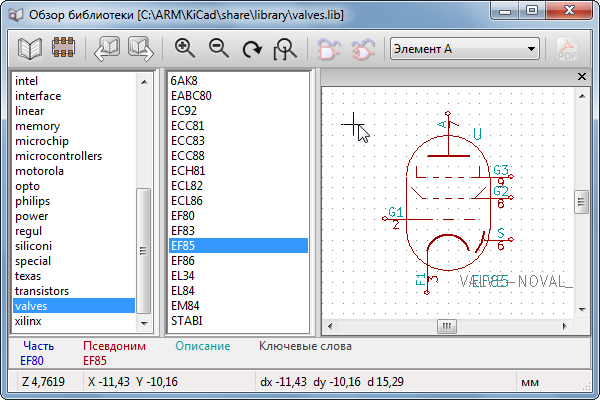
\includegraphics[height=0.5\textheight]{kicad/ee19.png}

  \end{enumerate} 
\end{itemize}

Вы также можете
вызвать обозреватель библиотек кнопкой\\
\menu{Просмотр библиотек и
компонентов}\ 
\includegraphics[height=2em]{kicad/ee20.png}

Выбрав элемент \dblms, вставьте символ в нужное место схемы \lms.
Позже вы сможете переместить его если нужно.
Зеркальное отражение компонента можно произвести следующим образом:

\begin{itemize}
  \item Поместите курсор на компоненте.
  \item По \rms\ выберите \menu{Ориентация компонента>Отражение}. 
  \item Без использования \term{контекстного меню}\ --- наведите мышь на
  компонент и нажмите кнопку \keys{X}\ или \keys{Y}.
\end{itemize}


% 
\secrel{\prog{eeschema}: редактор электрических схем}

обеспечивает:

\begin{itemize}
\item создание однолистовых и иерархических схем,
\item проверку их корректности ERC (контроль электрических правил),
\item создание списка электрических цепей netlist для редактора топологии платы
pcbnew или для spice-моделирования схемы, 
\item доступ к документации на используемые в схеме электронные компоненты
(datasheet).
\end{itemize}

% \secru{pcbnew\ --- редактор печатных плат}

обеспечивает:

\begin{itemize}
\item разработку плат, содержащих до 16 слоёв меди и до 12 технических слоёв
  (шелкография, паяльная маска и т. п.), 
\item выход на внешние трассировщики соединений посредством генерации описания 
платы на Specctra Design Language (on-line FreeRoute и др.),
\item генерацию технологических файлов для изготовления печатных плат
(Gerber-файлы для фотоплоттеров, файлы сверловок и файлы размещения компонентов), 
\item послойная печать схем и чертежей печатных плат на принтере или плоттере (в
форматах PostScript, HPGL, SVG и DXF), с рамкой формата или без неё.
\end{itemize}

% \secrel{\prog{gerbview}: просмотр фотошаблонов}

позволяет просматривать Gerber-файлы перед передачей печатных плат в
производство.

% \secru{cvpcb\ --- программа для выбора посадочных мест, соответствующих компонентам
% на схеме}
% \secru{wyoeditor\ --- текстовый редактор для просмотра отчётов}
% \section{Программа \prog{Wings3D} для создания 3D моделей}

Эта программа может вам пригодиться если вы планируете создавать 3D модели для PCB элементов.

Архив и файлы документации (Linux и Windows) в папке kicad/wings3d.

Взгляните на домашнюю страницу Wings3D чтобы узнать подробнее о программе.

pcbnew использует файлы в формате wrml (.wrl) экспортируемые из Wings3D (родной формат Wings3D - это .wings).

\subsection{Установка \prog{Wings3D} под \win}

\menu{\winr{\url{http://www.wings3d.com/}}>Downloads>Stable Release>\win
(32/64b)}

\menu{file{wings-n.n.n.exe}}

\menu{Compononets>\checkbox QuickLaunch>Next}

\menu{Location>\file{C:/Program Files/wings3d\_n.n.n}>Next>Install>Close}% 

% 
\chapter{Использование SPICE}
\cp{http://www.mithatkonar.com/wiki/doku.php/kicad/kicad\_spice\_quick\_guide}

\section{Доступные SPICE-пакеты}

\begin{itemize}
\item \href{http://ngspice.sourceforge.net/}{ngspice}: Arguably the most FOSSy
commonly available SPICE engine.
\item
\href{https://www.gnu.org/software/gnucap/}{gnucap}\note{уже включен в
виндозную сборку KiCAD}:
Not actually SPICE but tries to be syntax-compatible.
\item \href{http://www.spiceopus.si/}{SpiceOpus}: Proprietary but nice,
especially the output plotting.
\item \href{http://www.linear.com/designtools/software/}{LTSpice}: Linear
Technology's popular, proprietary Windows solution.
Works in \href{http://www.winehq.org/}{Wine}. Has a GUI anyway, so … ? Whether
it's scritable needs to be verified.
\item
\href{http://www.cadence.com/products/orcad/pspice_simulation/Pages/default.aspx}{PSpice}:
Windows-only, expensive, defacto standard professional solution in the USA. They
also have a tradition of making available a \emph{gratis} crippleware student
version.
Also has a \underline{GUI}, so … ?
\item \url{http://www.ngspice.com/}\ --- on-line вариант \prog{ngspice}, удобен
для начального обучения
\item Какие-то еще?
\end{itemize}

\section{Установка \prog{ngspice} под \win}

\menu{\winr\url{http://ngspice.sourceforge.net/download.html}>\prog{ng-spice-rework}>\file{ngspice-xx\_xxxxxx.zip}}

\section{Установка \prog{ngspice} под \linux}

\begin{verbatim}
root# aptitude install ngspice
\end{verbatim}

\section{Библиотеки компонентов со SPICE-элементами}

\begin{itemize}

\item There is a library of basic SPICE components that ships with KiCad. It's
good enough for initial experimentation.

\begin{itemize}
\item The library isn't included in Eeschema projects by default. You'll have to
add it manually if you want to use it.
In Debian-based Linux, it's at \\/usr/share/kicad/library/pspice.lib. (PSpice is
a popular proprietary version of SPICE.)
\end{itemize}

\item I am developing (very slowly)
\href{https://bitbucket.org/mithat/kicad-spice-library}{my own
library}\note{Mithat Konar \email{webs@mithatkonar.com}}
of components based on the above with some changes and additions.

\end{itemize}

\subsection{Настройка проекта}

\begin{enumerate}
\item Create a new project in the conventional way.
\item Open Eeschema and remove all the library references included by default.
\item Manually add one or more libraries with SPICE components to the project.
\begin{itemize}
  \item Note that the SPICE library that comes packaged with KiCad is not
  included by default in new KiCad projects.
\end{itemize}
\item Specify the SPICE engine you want to use:
\begin{itemize}
  \item Click the “Generate netlist” button (or the equivalent menu item).
  \item Select the “Spice” tab
  \item Enter the name of the command to invoke the simulator (with or without
path) in the “Simulator command:” textbox.
\end{itemize}
\end{enumerate}

\subsection{Making it happen}

\begin{enumerate}
  \item
Do your schematic capture, subject to a couple best practices:
\begin{itemize}
  \item
For named nets, use global labels instead of local labels.
\begin{itemize}
  \item
The reason for this is that in the netlists, global identifiers will be used
as-is but local labels get text prepended to the name—which makes it hard for
you to remember/guess what the full identifier is.
\end{itemize}
Use the ”0” component from a SPICE component library rather than the GND symbol.
\begin{itemize}
  \item
”0” is the official name of ground node in SPICE. Some engines may translate GND
into 0, some may not.
\end{itemize}
\end{itemize}
  \item
Specify the simulations you want to run and the output you want to display by
adding a text block (i.e., “comment”) with the needed SPICE and Nutmeg syntax
plus a little added mojo. To do an AC analysis and plot the response at node
\verb|vout|, you would add the following block:
\begin{lstlisting}
+PSPICE
.control
ac dec 66 1kHz 120kHz
plot vdb(vout)
set units = degrees
plot vp(vout)
.endc
\end{lstlisting}
\begin{itemize}
  \item
The line +PSPICE is KiCad-speak for, “Stick the following text at the end of a
SPICE netlist.”
\begin{itemize}
  \item
\textcircled{!} There appears to be a bug in the parser that requires you to add
a space after +PSPICE and before the line break.
\end{itemize}
  \item
There is a corresponding -PSPICE that is KiCad-speak for, “Stick the following
text at the start of a SPICE netlist.”
  \item
If you don't like seeing references to PSpice in your designs, you can use
+GNUCAP and -GNUCAP instead. I believe they are exact synonyms in this context,
but I am not certain.
  \item
Yes, this means you need to learn some
\href{http://newton.ex.ac.uk/teaching/cdhw/Electronics2/userguide/sec5.html}{SPICE
and Nutmeg} syntax. It's not hard.
\end{itemize}
  \item
Run the simulation:
\begin{itemize}
  \item
Click the “Generate netlist” button (or the equivalent menu item).
  \item
Select the “Spice” tab, and make sure “Default format” is checked. (You should
only have to do this once; it will just save you time in subsequent invocations
of the dialog.)
  \item
Click the “Run simulator” button.
\end{itemize}
\end{enumerate}

% 
% \secup